\chapter{IDENTITY OF PARTICLES}\label{IDENTITY OF PARTICLES}
\section{The principle of indistinguishability of similar particles}\label{The principle of indistinguishability of similar particles}
IN classical mechanics, identical particles (electrons, say) do not lose their “individuality”, despite the identity of their physical properties. For we can imagine the particles at some instant to be “numbered”, and follow the subsequent motion of each of these in its path; then at any instant the particles can be identified.

In quantum mechanics the situation is entirely different. We have already mentioned several times that, by virtue of the uncertainty principle, the concept of the path of an electron ceases to have any meaning. If the position of an electron is exactly known at a given instant, its coordinates have no definite values even at the next instant. Hence, by localizing and numbering the electrons at some instant, we make no progress towards identifying them at subsequent instants; if we localize one of the electrons, at some other instant, at some point in space, we cannot say which of the electrons has arrived at this point.

Thus, in quantum mechanics, there is in principle no possibility of separately following each of a number of similar particles and thereby distinguishing them. We may say that, in quantum mechanics, identical particles entirely lose their “individuality”. The identity of the particles with respect to their physical properties is here very far-reaching: it results in the complete indistinguishability of the particles.

This principle of the \textit{indistinguishability of similar particles}, as it is called, plays a fundamental part in the quantum theory of systems composed of identical particles. Let us start by considering a system of only two particles. Because of the identity of the particles, the states of the system obtained from each other by merely interchanging the two particles must be completely equivalent physically. This means that, as a result of this interchange, the wave function of the system can change only by an unimportant phase factor. Let $ \psi(\xi_1,\xi_2) $ be the wave function of the system, $ \xi_1 $ and $ \xi_2 $ conventionally denoting the three coordinates and the spin projection for each particle. Then we must have
\[ \psi(\xi_1,\xi_2)=\e^{\i\alpha}\psi(\xi_2,\xi_1), \]
where $\alpha$ is some real constant. By repeating the interchange, we return to the original state, while the function $\psi$ is multiplied by $ \e^{2\i\alpha} $. Hence it follows that $ \e^{2\i\alpha}=1 $, or $ \e^{\i\alpha}=\pm1 $. Thus
\[ \psi(\xi_1,\xi_2)=\pm\psi(\xi_2,\xi_1). \]



We thus reach the result that there are only two possibilities: the wave function is either \textit{symmetrical} (i.e. it is unchanged when the particles are interchanged) or \textit{antisymmetrical} (i.e. it changes sign when this interchange is made). It is obvious that the wave functions of all the states of a given system must have the same symmetry; otherwise, the wave function of a state which was a superposition of states of different symmetry would be neither symmetrical nor antisymmetrical.

This result can be immediately generalized to systems consisting of any number of identical particles. For it is clear from the identity of the particles that, if any pair of them has the property of being described by, say, symmetrical wave functions, any other pair of such particles has the same property. Hence the wave function of identical particles must either be unchanged when any pair of particles are interchanged (and hence when the particles are permuted in any manner), or change sign when any pair are interchanged. In the first case we speak of a \textit{symmetrical} wave function, and in the second case of an \textit{antisymmetrical} one.

The property of being described by symmetrical or antisymmetrical wave functions depends on the nature of the particles. Particles described by antisymmetrical functions are said to obey \textit{Fermi–Dirac statistics} (or to be \textit{fermions}), while those which are described by symmetrical functions are said to obey \textit{Bose-Einstein statistics} (or to be \textit{bosons}).\footnote{This terminology refers to the statistics which describes a perfect gas composed of particles with antisymmetrical and symmetrical wave functions respectively. In actual fact we are concerned here not only with a different statistics, but essentially with a different mechanics. Fermi statistics was proposed by E. Fermi for electrons in 1926, and its relation to quantum mechanics was elucidated by P. A. M. Dirac (1926). Bose statistics was proposed by S. N. Bose for light quanta, and generalized by A. Einstein (1924).}

From the laws of relativistic quantum mechanics it can be shown (see RQT, \S25) that the statistics obeyed by particles is uniquely related to their spin: particles with half-integral spin are fermions, and those with integral spin are bosons.

The statistics of complex particles is determined by the parity of the number of elementary fermions entering into their composition. For an interchange of two identical complex particles is equivalent to the simultaneous interchange of several pairs of identical elementary particles. The interchange of bosons does not change the wave function, while the interchange of fermions changes its sign. Hence complex particles containing an odd number of elementary fermions obey Fermi statistics, while those containing an even number obey Bose statistics. This result is, of course, in agreement with the above rule, since a complex particle has an integral or a half-integral spin according as the number of particles with half-integral spin entering into its composition is even or odd.

Thus atomic nuclei of odd atomic weight (i.e. containing an odd number of neutrons and protons) obey Fermi statistics, and those of even atomic weight obey Bose statistics. For atoms, which contain both nuclei and electrons, the statistics is evidently determined by the parity of the sum of the atomic weight and the atomic number.

Let us consider a system composed of $ N $ identical particles, whose mutual interaction can be neglected. Let $ \psi_1, \psi_2, \dots $ be the wave functions of the various stationary states which each of the particles separately may occupy. The state of the system as a whole can be defined by giving the numbers of the states which the individual particles occupy. The question arises how the wave function $\psi$ of the whole system should be constructed from the functions $ \psi_1, \psi_2, \dots $.

Let $ p_1, p_2, \dots, p_N $ be the numbers of the states occupied by the individual particles (some of these numbers may be the same). For a system of bosons, the wave function $ \psi(\xi_1, \xi_2, \dots, \xi_N) $ is given by a sum of products of the form
\begin{equation}\label{61.1}
\psi_{p_1}(\xi_1)\psi_{p_2}(\xi_2)\dots\psi_{p_n}(\xi_N),
\end{equation}
with all possible permutations of the different suffixes $ p_1, p_2, \dots $; this sum clearly possesses the required symmetry property. For example, for a system of two particles in different states ($ p_1 \ne p_2 $),
\begin{equation}\label{61.2}
\psi(\xi_1,\xi_2)=\frac{1}{\sqrt{2}}\left[\psi_{p_1}(\xi_1)\psi_{p_2}(\xi_2)+\psi_{p_1}(\xi_2)\psi_{p_2}(\xi_1) \right].
\end{equation}



The factor $ 1/\sqrt{2} $ is introduced for normalization purposes; all the functions $ \psi_1, \psi_2, \dots $ are orthogonal and are supposed normalized.

In the general case of a system containing an arbitrary number $ N $ of particles, the normalized wave function is
\begin{equation}\label{61.3}
\psi_{N_1N_2\dots}=\left(\frac{N_1!N_2!\dots}{N!} \right)^{1/2}\sum\psi_{p_1}(\xi_1)\psi_{p_2}(\xi_2)\dots\psi_{p_N}(\xi_N),
\end{equation}
where the sum is taken over all permutations of the different suffixes $ p_1, p_2, \dots, p_N $ and the numbers $ N_i $ show how many of these suffixes have the same value $ i $ (with $ \sum N_i = N $). In the integration of $ |\psi|^2 $ over $ \xi_1, \xi_2, \dots, \xi_N $, all terms vanish except the squared modulus of each term of the sum;\footnote{The integration over $ \xi $ is conventionally understood in \S\S\ref{Symmetry with respect to interchange}–\ref{Second quantization. The case of Fermi statistics} as including integration over the coordinates and summation over $\sigma$.
} since the total number of terms in the sum \eqref{61.3} is evidently $ N!/(N_1!N_2!\dots) $, the normalization factor in \eqref{61.3} is obtained.

For a system of fermions, the wave function $\psi$ is an antisymmetrical combination of the products \eqref{61.1}. For a system of two particles we have
\begin{equation}\label{61.4}
\psi(\xi_1,\xi_2)=\frac{1}{\sqrt{2}}\left[\psi_{p_1}(\xi_1)\psi_{p_2}(\xi_2)-\psi_{p_1}(\xi_2)\psi_{p_2}(\xi_1) \right].
\end{equation}
For the general case of N particles, the wave function can be written in the form of a determinant
\begin{equation}\label{61.5}
\psi_{N_1N_2\dots}=\frac{1}{\sqrt{N!}}\left|\begin{array}{cccc}
\psi_{p_1}(\xi)&\psi_{p_1}(\xi_2)&\dots&\psi_{p_1}(\xi_N)\\
\psi_{p_2}(\xi)&\psi_{p_2}(\xi_2)&\dots&\psi_{p_2}(\xi_N)\\
\dots&\dots&\dots&\dots\\
\psi_{p_N}(\xi)&\psi_{p_N}(\xi_2)&\dots&\psi_{p_N}(\xi_N)\\
\end{array}   \right|.
\end{equation}
Here an interchange of two particles corresponds to an interchange of two columns of the determinant, as a result of which the latter changes sign.

The following important result is a consequence of the expression \eqref{61.5}. If among the numbers $ p_1, p_2, \dots $ two are the same, two rows of the determinant are the same, and it therefore vanishes identically. It will be different from zero only when all the numbers $ p_1, p_2, \dots $ are different. Thus, in a system consisting of identical fermions, no two (or more) particles can be in the same state at the same time. This is called \textit{Pauli’s principle} (1925).
\section{Exchange interaction}\label{Exchange interaction}
The fact that Schr\"odinger’s equation does not take account of the spin of particles does not invalidate this equation or the results obtained by means of it. This is because the electrical interaction of the particles does not depend on their spins.\footnote{This is true only so long as we consider the non-relativistic approximation. When relativistic effects are taken into account, the interaction of charged particles does depend on their spin.
} Mathematically, this means that the Hamiltonian of a system of electrically interacting particles (in the absence of a magnetic field) does not contain the spin operators, and hence, when it is applied to the wave function, it has no effect on the spin variables. Hence Schr\"odinger’s equation is actually satisfied by each component of the wave function; in other words, the wave function of the system of particles can be written in the form of a product
\[ \psi(\xi_1,\xi_2)=\chi(\sigma_1,\sigma_2,\dots)\phi(\bm{r}_1,\bm{r}_2,\dots), \]
where the function $\phi$ depends only on the coordinates of the particles and the function $\chi$ only on their spins. We call the former a \textit{coordinate} or \textit{orbital} wave function, and the latter a \textit{spin} wave function. Schr\"odinger’s equation essentially determines only the coordinate function $\phi$, the function $\chi$ remaining arbitrary. In any instance where we are not interested in the actual spin of the particles, we can therefore use Schr\"odinger’s equation and regard as the wave function the coordinate function alone, as we have done hitherto.

However, despite the fact that the electrical interaction of the particles is independent of their spin, there is a peculiar dependence of the energy of the system on its total spin, arising ultimately from the principle of indistinguishability of similar particles.

Let us consider a system consisting of only two identical particles. By solving Schr\"odinger’s equation we find a series of energy levels, to each of which there corresponds a definite symmetrical or antisymmetrical coordinate wave function $ \phi(\bm{r}_1, \bm{r}_2) $. For, by virtue of the identity of the particles, the Hamiltonian (and therefore the Schr\"odinger’s equation) of the system is invariant with respect to interchange of the particles. If the energy levels are not degenerate, the function $ \phi(\bm{r}_1, \bm{r}_2) $ can change only by a constant factor when the coordinates $ \bm{r}_1 $ and $ \bm{r}_2 $ are interchanged; repeating this interchange, we see that this factor can only be\footnote{When there is degeneracy we can always choose linear combinations of the functions belonging to a given level, such that this condition is again satisfied.
} $ \pm1 $.

Let us first suppose that the particles have zero spin. The spin factor for such particles is absent altogether, and the wave function reduces to the coordinate function $ \phi(\bm{r}_1, \bm{r}_2) $, which must be symmetrical (since particles with zero spin obey Bose statistics). Thus not all the energy levels obtained by a formal solution of Schr\"odinger’s equation can actually exist; those to which antisymmetrical functions $\phi$ correspond are not possible for the system under consideration.

The interchange of two similar particles is equivalent to the operation of inversion of the coordinate system (the origin being taken to bisect the line joining the two particles). On the other hand, the result of inversion is to multiply the wave function $\phi$ by $ (-1)^l $, where $ l $ is the orbital angular momentum of the relative motion of the two particles (see \S\ref{Parity of a state}). By comparing these considerations with those given above, we conclude that a system of two identical particles with zero spin can have only an even orbital angular momentum.

Next, let the system consist of two particles with spin $ 1/2 $ (say, electrons). Then the complete wave function of the system (i.e. the product of the function $ \phi(\bm{r}_1, \bm{r}_2) $ and the spin function $ \chi(\sigma_1,\sigma_2) $) must certainly be antisymmetrical with respect to an interchange of the two particles. Hence, if the coordinate function is symmetrical, the spin function must be antisymmetrical, and vice versa. We shall write the spin function in spinor form, i.e. as a spinor $ \chi^{\lambda\mu} $ of rank two, each of whose indices corresponds to the spin of one of the electrons. A symmetrical spinor ($ \chi^{\lambda\mu} = \chi^{\mu\lambda} $) corresponds to a function symmetrical with respect to the spins of the two particles, and an antisymmetrical spinor ($ \chi^{\lambda\mu} = -\chi^{\mu\lambda} $) to an antisymmetrical function. We know, however, that a symmetrical spinor of rank two describes a system with total spin unity, while an antisymmetrical spinor reduces to a scalar, corresponding to zero spin.

Thus we reach the following conclusion. The energy levels to which there correspond symmetrical solutions $ \phi(\bm{r}_1, \bm{r}_2) $ of Schr\"odinger’s equation can actually occur when the total spin of the system is zero, i.e. when the spins of the two electrons are “antiparallel”, giving a sum of zero. The values of the energy belonging to antisymmetrical functions $ \phi(\bm{r}_1, \bm{r}_2) $, on the other hand, require a value of unity for the total spin, i.e. the spins of the two electrons must be “parallel”.

In other words, the possible values of the energy of a system of electrons depend on their total spin. For this reason we can speak of a peculiar interaction of the particles which results in this dependence. This is called \textit{exchange interaction}. It is a purely quantum effect, which entirely vanishes (like the spin itself) in the passage to the limit of classical mechanics.

The following situation is characteristic of the case of a system of two electrons which we have discussed. To each energy level there corresponds one definite value of the total spin, $ 0 $ or $ 1 $. This one-to-one correspondence between the spin values and the energy levels is preserved, as we shall see below (\S\ref{Symmetry with respect to interchange}), in systems containing any number of electrons. It does not hold, however, for systems composed of particles whose spin exceeds $ 1/2 $.

Let us consider a system of two particles, each with arbitrary spin $ s $. Its spin wave function is a spinor of rank $ 4s $:
\[ \chi^{\overbrace{\lambda\mu\dots}^{2s}\overbrace{\rho\sigma}^{2s}}, \]
half ($ 2s $) of whose indices correspond to the spin of one particle, and the other half to that of the other particle. The spinor is symmetrical with respect to the indices in each group. An interchange of the two particles corresponds to an interchange of all the indices $ \lambda,\mu,\dots $ of the first group with the indices $ \rho, \sigma, \dots $ of the second group. In order to obtain the spin function of a state of the system with total spin $ S $, we must contract this spinor with respect to $ 2s - S $ pairs of indices (each pair containing one index from $ \lambda,\mu,\dots $ and one from $ \rho, \sigma, \dots $), and symmetrize it with respect to the remainder; as a result we obtain a symmetrical spinor of rank $ 2S $. However, the contraction of a spinor with respect to a pair of indices means, as we know, the construction of a combination antisymmetrical with respect to these indices. Hence, when the particles are interchanged, the spin wave function is multiplied by $ (-1)^{2s-S} $.

On the other hand, the complete wave function of a system of two particles must be multiplied by $ (-1)^{2s} $ when they are interchanged (i.e. by $ +1 $ for integral $ s $ and by $ -1 $ for half-integral $ s $). Hence it follows that the symmetry of the coordinate wave function with respect to an interchange of the particles is given by the factor $ (-1)^S $, which depends only on $ S $. Thus we reach the result that the coordinate wave function of a system of two identical particles is symmetrical when the total spin is even, and antisymmetrical when it is odd.

Recalling what was said above concerning the relation between interchange of the particles and inversion of the coordinate system, we conclude also that, when the spin $ S $ is even (odd), the system can have only an even (odd) orbital angular momentum.

We see that here also a certain dependence is revealed between the possible values of the energy of the system and the total spin, but this dependence is not necessarily one-to-one. The energy levels to which there correspond symmetrical (antisymmetrical) coordinate wave functions can occur for any even (odd) value of $ S $.

Let us calculate how many different states of the system there are with even and odd S. The quantity $ S $ takes $ 2s + 1 $ values: $ 2s, 2s - 1, \dots 0 $. For any given $ S $ there are $ 2S + 1 $ states differing in the value of the $ z $-component of the spin ($ (2s+1)^2 $ different states altogether). Let $ s $ be integral. Then, among the $ 2s + 1 $ values of $ S $, $ s + 1 $ are even and $ s $ odd. The total number of states with even $ S $ is equal to the sum
\[ \sum_{S=0,2,\dots,2s}(2S+1)=(2s+1)(s+1); \]
the remaining $ s (2s+1) $ states have odd $ S $. Similarly, we find that, when $ s $ is half-integral, there are $ s (2s+1) $ states with even values of $ S $ and $ (s+1)(2s+1) $ with odd values.





{\small
\textbf{PROBLEMS}


\textbf{1.} Determine the exchange splitting of the energy levels of a system of two electrons, regarding the interaction of the electrons as a perturbation.





SOLUTION. Let the particles be (when their interaction is neglected) in states with orbital wave functions $ \phi_1(\bm{r}_1) $ and $ \phi_2(\bm{r}_2) $. The states of the system with total spin $ S = 0 $ and $ S = 1 $ correspond to symmetrized and antisymmetrized products respectively:
\[ \phi=\frac{1}{\sqrt{2}}\left[\phi_1(\bm{r}_1)\phi_2(\bm{r}_2)\pm\phi_1(\bm{r}_2)\phi_2(\bm{r}_1) \right]. \]
The mean value of the operator of the interaction $ U (\bm{r}_2-\bm{r}_1) $ of the particles in these states is $ A\pm J $, where
\[ A=\iint U|\phi_1(\bm{r}_1)|^2|\phi_2(\bm{r}_2)|^2\d V_1\d V_2, \]
\[ J=\iint U\phi_1(\bm{r}_1)\phi_1^*(\bm{r}_2)\phi_2(\bm{r}_2)\phi_2^*(\bm{r}_1)\d V_1\d V_2 \]
the latter being called the \textit{exchange integral}. Omitting the additive constant $ A $, which is not an exchange term, we therefore find the level shifts $ \Delta E_0 = J, \Delta E_1 = -J $ (where the suffix indicates the value of $ S $). These quantities can be represented as the eigenvalues of the spin \textit{exchange operator}\footnote{First used by Dirac.}
\begin{equation}\label{62-1-1}
\hat{V}_{\text{exch}}=-(1/2)J(1+4\hat{\bm{s}}_1\hat{\bm{s}}_2)\tag{1}
\end{equation}
the eigenvalues of the product $\hat{\bm{s}}_1\hat{\bm{s}}_2  $ are derived in \S\ref{Spinors}, Problem $ 2 $.

If the electrons belong to different atoms, for example, the exchange integral decreases exponentially with increasing distance $ R $ between the atoms. It is clear from the form of the integrand that this integral is determined by the “overlap” of the wave functions of the states $\phi_1(\bm{r}_1) $ and $ \phi_2(\bm{r}_2) $; using the asymptotic law of decrease of the wave functions of states of a discrete spectrum (cf. \eqref{21.6}), we find that
\[ J\sim\exp(-(\varkappa_1+\varkappa_2)R),\quad\varkappa_1=\frac{1}{\h}\sqrt{2m|E|},\quad\varkappa_2=\frac{1}{\h}\sqrt{2m|E_2|}, \]
where $ E_1 $ and $ E_2 $ are the energy levels of the electron in the two atoms.





\textbf{2.} The same as Problem $ 1 $, but for a system of three electrons.





SOLUTION. Using formula \eqref{62-1-1}, Problem $ 1 $, we can write the operator of pairwise exchange interaction in a system of three electrons as
\begin{equation}\label{62-2-1}
\hat{V}_{\text{exch}}=-\sum J_{ab}(1/2+2\hat{\bm{s}}_a\hat{\bm{s}}_b)\tag{1}
\end{equation}
where the summation is over pairs of particles $ 12 $, $ 13 $ and $ 23 $. The matrix elements of the operators $ \hat{\bm{s}}_a\hat{\bm{s}}_b $ between states with different values of the pair of numbers $ \sigma_a, \sigma_b $ are given by formulae \eqref{55.6} as
\[ \<1/2,1/2|\bm{s}_a\bm{s}_b|1/2,1/2\>=1/4,\quad\<1/2,-1/2|\bm{s}_a\bm{s}_b|1/2,-1/2\>=-1/4, \]
\[ \<1/2,-1/2|\bm{s}_a\bm{s}_b|-1/2,1/2\>=1/2. \]


We first determine the energy corresponding to the greatest possible value of the total-spin component $ M_s = \sigma_1+\sigma_2+\sigma_3 $, viz. $ M_s = 3/2 $. This gives the energy of the state with total spin $ S = 3/2 $. On calculating the corresponding diagonal matrix element of the operator \eqref{62-2-1}, we find
\[ \Delta E_{3/2}=-(J_{12}+J_{13}+J_{23}). \]



Next we take states with $ M_s = 1/2 $ This value can occur in three ways, depending on which of the numbers $ \sigma_1, \sigma_2, \sigma_3 $ is $ -1/2 $ (the other two being $ 1/2 $). Thus for these states we should have a secular equation of the third degree. The calculation can, however, be simplified immediately by noting that one of the roots of this equation must correspond to the energy already found for the state with $ S = 3/2 $, and the secular equation must therefore have the factor $ \Delta E-\Delta E_{3/2} $. In this way the calculation of the free term in the cubic equation can be avoided.\footnote{This device is particularly useful in similar calculations for systems with a larger number of particles.
}

The leading terms of the equation are found to be
\begin{multline*}
(\Delta E)^3+(J_{12}+J_{13}+J_{23})(\Delta E)^2+\\
+ [J_{12}J_{13}+J_{12}J_{23}+J_{13}J_{23}-(J_{12}^2+J_{13}^2+J_{23}^2)]\Delta E+\dots=0,
\end{multline*}
Dividing by $ \Delta E+J_{12}+J_{13}+J_{23} $, we find the two energy levels corresponding to states with spins $ S =1/2  $:
\[ \Delta E_{1/2}=\pm[J_{12}^2+J_{13}^2+J_{23}^2-J_{12}J_{13}-J_{12}J_{23}-J_{13}J_{23}]^{1/2}. \]
Thus there are three energy levels, in accordance with the calculation in \S\ref{Symmetry with respect to interchange}, Problem 1





\textbf{3.} In which states can the $ {}^8\mathrm{Be} $ nucleus decay into two $\alpha$-particles?





SOLUTION. Since the $\alpha$-particle has no spin, a system of two α-particles can only have an even orbital angular momentum (equal to the total angular momentum), and its states are even. The decay in question is therefore possible only from even states of the $ {}^8\mathrm{Be} $ nucleus with even total angular momentum.}
\section{Symmetry with respect to interchange}\label{Symmetry with respect to interchange}
By considering a system composed of only two particles, we have been able to show that its coordinate wave functions $ \phi(\bm{r}_1, \bm{r}_2) $ for the stationary states must be either symmetrical or antisymmetrical. In the general case of a system of an arbitrary number of particles, the solutions of Schr\"odinger’s equation (the coordinate wave functions) need not necessarily be either symmetrical or antisymmetrical with respect to the interchange of any pair of particles, as the complete wave functions (which include the spin factor) must be. This is because an interchange of only the coordinates of two particles does not correspond to a physical interchange of them. The physical identity of the particles here leads only to the fact that the Hamiltonian of the system is invariant with respect to the interchange of the particles, and hence, if some function is a solution of Schr\"odinger’s equation, the functions obtained from it by various interchanges of the variables will also be solutions.

Let us first of all make some remarks regarding interchanges in general. In a system of $ N $ particles, $ N! $ different permutations in all are possible. If we imagine all the particles to be numbered, each permutation can be represented by a definite sequence of the numbers $ 1, 2, 3, \dots $. Every such sequence can be obtained from the natural sequence $ 1, 2, 3, \dots $ by successive interchanges of pairs of particles. The permutation is called even or odd, according as it is brought about by an \textit{even} or \textit{odd} number of such interchanges. We denote by the $ \hat{P} $ operators of permutations of $ N $ particles, and introduce a quantity $ \delta P $ which is $ +1 $ if is an even permutation and $ -1 $ if it is odd. If $\phi$ is a function symmetrical with respect to all the particles, we have
\[ \hat{P}\phi=\phi, \]
while, if $\phi$ is antisymmetrical with respect to all the particles, then
\[ \hat{P}\phi=\delta_P\phi. \]



From an arbitrary function $ \phi(\bm{r}_1, \bm{r}_2, …\dots, \bm{r}_N) $, we can form a symmetrical function by the operation of \textit{symmetrization}, which can be written
\begin{equation}\label{63.1}
\phi_{\text{sym}}=\mathrm{const}\sum_P\hat{P}\phi,
\end{equation}
where the summation extends over all possible permutations. The formation of an antisymmetrical function (an operation sometimes called \textit{alternation}) can be written as
\begin{equation}\label{63.2}
\phi_{\mathrm{ant}}=\mathrm{const}\sum_P\delta_P\hat{P}_\phi.
\end{equation}



Let us return to considering the behaviour, with respect to permutations, of the wave functions $\phi$ of a system of identical particles.\footnote{From the mathematical point of view, the problem is to find irreducible representations of the permutation group. A detailed account of the mathematical theory of permutation (or symmetry) groups is given by H. Weyl, \textit{The Theory of Groups and Quantum Mechanics}, Methuen, London 1931; M. Hamermesh, \textit{Group Theory and its Application to Physical Problems}, Pergamon, London, 1962; I. G. Kaplan, \textit{Symmetry of Many-Electron Systems}, Academic Press, New York, 1974.
} The fact that the Hamiltonian $\hat{H}$ of the system is symmetrical with respect to all the particles means, mathematically, that $\hat{H}$ commutes with all the permutation operators $ \hat{P} $. These operators, however, do not commute with one another, and so they cannot be simultaneously brought into diagonal form. This means that the wave functions $\phi$ cannot be so chosen that each of them is either symmetrical or antisymmetrical with respect to all interchanges separately.\footnote{Except for a system of only two particles, where there is a single interchange operator, which can be brought into diagonal form simultaneously with the Hamiltonian.
}

Let us try to determine the possible types of symmetry of the functions $ \phi(\bm{r}_1, \bm{r}_2, \dots, \bm{r}_N) $ of $ N $ variables (or of sets of several such functions) with respect to permutations of the variables. The symmetry must be such that it cannot be increased, i.e. such that any additional operation of symmetrization or alternation, on being applied to these functions, would reduce them either to linear combinations of themselves or to zero identically.

We already know two operations which give functions with the greatest possible symmetry: symmetrization with respect to all the variables, and alternation with respect to all the variables. These operations can be generalized as follows.

We divide the set of all the $ N $ variables $ \bm{r}_1, \bm{r}_2, \dots, \bm{r}_N $ (or, what is the same thing, the suffixes $ 1, 2, 3, \dots, N $) into several sets, containing $ N_1, N_2, \dots $ elements (variables); $ N_1+N_2+ \dots = N $. This division can be conveniently shown by a diagram (known as a \textit{Young diagram}) in which each of the numbers $ N_1, N_2, \dots $ is represented by a line of several cells (thus, Fig. 21 gives a diagram of the divisions $ 6+4+4+3+3+1+1 $ and $ 7+5+5+3+1+1 $ for $ N = 22 $); one of the numbers $ 1, 2, 3, \dots $ is to be placed in each square. If we place the lines in order of decreasing length (as in Fig. \ref{Fig.21}), the diagram contains not only successive horizontal rows, but also vertical columns.



Let us symmetrize an arbitrary function $ \phi(\bm{r}_1, \bm{r}_2, \bm{r}_N) $ with respect to the variables in each row. The alternation operation can then be performed only
\begin{wrapfigure}[9]{l}[0cm]{0cm}
	
\begin{tikzpicture}[scale=0.45]
	\draw (0,0)--(6,0);
	\draw (0,-1)--(6,-1);
	\draw (0,-2)--(4,-2);
	\draw (0,-3)--(4,-3);
	\draw (0,-4)--(3,-4);
	\draw (0,-5)--(3,-5);
	\draw (0,-6)--(1,-6);
	\draw (0,-7)--(1,-7);
	\draw (0,0)--(0,-7);
	\draw (1,0)--(1,-7);
	\draw (2,0)--(2,-5);
	\draw (3,0)--(3,-5);
	\draw (4,0)--(4,-3);
	\draw (5,0)--(5,-1);
	\draw (6,0)--(6,-1);
	\draw (8,0)--(15,0);
	\draw (8,-1)--(15,-1);
	\draw (8,-2)--(13,-2);
	\draw (8,-3)--(13,-3);
	\draw (8,-4)--(11,-4);
	\draw (8,-5)--(9,-5);
	\draw (8,-6)--(9,-6);
	\draw (8,0)--(8,-6);
	\draw (9,0)--(9,-6);
	\draw (10,0)--(10,-4);
	\draw (11,0)--(11,-4);
	\draw (12,0)--(12,-3);
	\draw (13,0)--(13,-3);
	\draw (14,0)--(14,-1);
	\draw (15,0)--(15,-1);
	\end{tikzpicture}\caption{FIG.21}\label{Fig.21}
\end{wrapfigure}
with respect to the variables in different rows; alternation with respect to a pair of variables in the same row clearly gives zero identically.

Having chosen one variable from each row, we can, without loss of generality, regard them as being in the first cells in each row (after symmetrization, the order of the variables among the cells in each row is immaterial); let us alternate with respect to these variables. Having then deleted the first column, we alternate with respect to variables chosen one from each row in the thus “curtailed” diagram; these variables can again be regarded as being in the first cells of the “curtailed” rows. Continuing this process, we finally have the function first symmetrized with respect to the variables in each row and then alternated with respect to the variables in each column. After alternation, of course, the function in general ceases to be symmetrical with respect to the variables in each row. The symmetry is preserved only with respect to the variables in the cells of the first row which project beyond the other rows.

Having distributed the $ N $ variables in various ways among the rows of a Young diagram (the distribution among the cells in each row is immaterial), we thus obtain a series of functions, which are transformed linearly into one another when the variables are permuted in any manner.\footnote{It would be possible to perform the symmetrization and alternation in the reverse order: to alternate with respect to the variables in each column, and then to symmetrize with respect to those in the rows. This, however, would give effectively the same thing, since the functions obtained by the two methods are linear combinations of one another.
} However, it must be emphasized that not all these functions are linearly independent; the number of independent functions is in general less than the number of possible distributions of the variables among the rows of the diagram. We shall not pause here, however, to discuss this more closely.\footnote{The independent functions that are transformed into linear combinations of one another form the basis of an irreducible representation of the permutation group. Their number is the dimension of the representation. For particles with spin $ 1/2 $ the number is derived in Problem $ 1 $ below.}

Thus any Young diagram determines some type of symmetry of functions with respect to permutations. By constructing all the possible Young diagrams (for a given $ N $), we find all possible types of symmetry. This amounts to dividing the number N in all possible ways into a sum of smaller terms, including the number $ N $ itself; thus for $ N = 4 $ the possible partitions are $ 4, 3+1, 2+2, 2+1+1, 1+1+1+1 $.

To each energy level of the system we can make correspond a Young diagram which determines the permutational symmetry of the appropriate solutions of Schr\"odinger’s equation; in general, several different functions correspond to each value of the energy, and these are transformed linearly into each other by permutations. The existence of this “permutational degeneracy” is related to the fact that the operators $ \hat{P} $ each commute with the Hamiltonian but not with one another (see the middle of \S\ref{Stationary states}). However, it must be emphasized that this does not signify any additional physical degeneracy of the energy levels. All these different coordinate wave functions, multiplied by the spin functions, enter into a single definite combination—the complete wave function—which satisfies (according to the spin of the particles) the condition of symmetry or antisymmetry.

Among the various types of symmetry there are always (for any given $ N $) two to each of which only one function corresponds. One of these corresponds to a function symmetrical with respect to all the variables, and the other to one which is similarly antisymmetrical; in the first case, the Young diagram consists of a single row of $ N $ cells, and in the second case of a single column.

Let us now consider the spin wave functions $ \chi(\sigma_1, \sigma_2, \dots, \sigma_N) $. Their kinds of symmetry with respect to permutations of the particles are given by the same Young diagrams, with the components of the spins of the particles taking the part of variables. There arises the question of what diagram must correspond to the spin function for a given diagram of the coordinate function. Let us first suppose that the spin of the particles is integral. Then the complete wave function $\psi$ must be symmetrical with respect to all the particles. For this to be so, the symmetry of the spin and coordinate functions must be given by the same Young diagram, and the complete wave function $\psi$ is expressed as definite bilinear combinations of the two; we shall not here pause to examine more closely the problem of constructing these combinations.

Next, suppose the spin of the particles to be half-integral. Then the complete wave function must be antisymmetrical with respect to all the particles. It can be shown that, for this to be so, the Young diagrams for the coordinate and spin functions must be in dual relation, i.e. obtained from each other by interchanging rows and columns (as in the two diagrams shown in Fig. \ref{Fig.21})

Let us consider in more detail the important case of particles with spin $ 1/2 $ (electrons, for instance). Each of the spin variables $ \sigma_1, \sigma_2, \dots $ here takes only the two values $ \pm1/2 $. Since a function antisymmetrical with respect to any two variables vanishes when these variables take the same value, it is clear that the function $\chi$ can be alternated only with respect to pairs of variables; if we alternate with respect to even three variables, two of them must always take the same value, so that we have zero identically.

Thus, for a system of electrons, the Young diagrams for the spin functions can contain columns of only one or two cells (i.e. only one or two rows); in the Young diagrams for the coordinate functions, the same is true of the number of columns. The number of possible types of permutational symmetry for a system of $ N $ electrons is therefore equal to the number of possible partitions of the number $ N $ into a sum of ones and twos. When $ N $ is even, this number is $ N/2+1 $ (partitions with $ 0, 1, \dots, N/2 $ twos), while if $ N $ is odd it is $ (N+1)/2 $ (partitions with $ 0, 1, \dots, (N-1)/2 $ twos). Thus, for instance, Fig. \ref{Fig.22} shows the possible Young diagrams (coordinate and spin) for $ N = 4 $.








It is easy to see that each of these types of symmetry (i.e. each of the Young diagrams) corresponds to a definite total spin $ S $ of the system of electrons. We shall consider the spin functions in spinor form, i.e. as spinors $ \chi^{\lambda\mu\dots} $ of rank $ N $, whose indices (each of which corresponds to the spin of an individual particle) will be the variables that are arranged in the cells of the
\begin{wrapfigure}[10]{r}[0cm]{0cm}
	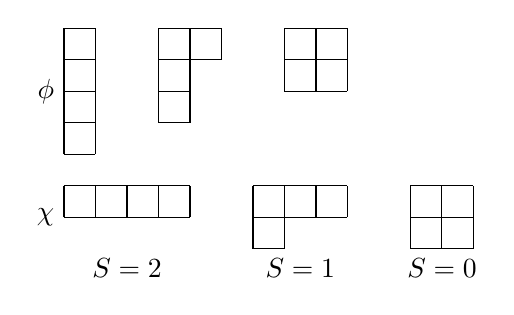
\begin{tikzpicture}[scale=0.4]
	\draw (6,0)--(7,0);
	\draw (11,0)--(13,0);
	\draw (0,1)--(4,1);
	\draw (6,1)--(9,1);
	\draw (11,1)--(13,1);
	\draw (0,2)--(4,2);
	\draw (6,2)--(9,2);
	\draw (11,2)--(13,2);
	\draw (0,3)--(1,3);
	\draw (0,4)--(1,4);
	\draw (3,4)--(4,4);
	\draw (0,5)--(1,5);
	\draw (3,5)--(4,5);
	\draw (7,5)--(9,5);
	\draw (0,6)--(1,6);
	\draw (3,6)--(5,6);
	\draw (7,6)--(9,6);
	\draw (0,7)--(1,7);
	\draw (3,7)--(5,7);
	\draw (7,7)--(9,7);
	\draw (0,1)--(0,2);
	\draw (0,3)--(0,7);
	\draw (1,1)--(1,2);
	\draw (1,3)--(1,7);
	\draw (2,1)--(2,2);
	\draw (3,1)--(3,2);
	\draw (3,4)--(3,7);
	\draw (4,1)--(4,2);
	\draw (4,4)--(4,7);
	\draw (5,6)--(5,7);
	\draw (6,0)--(6,2);
	\draw (7,0)--(7,2);
	\draw (7,5)--(7,7);
	\draw (8,1)--(8,2);
	\draw (8,5)--(8,7);
	\draw (9,1)--(9,2);
	\draw (9,5)--(9,7);
	\draw (11,0)--(11,2);
	\draw (12,0)--(12,2);
	\draw (13,0)--(13,2);
	\node[below] at (2,0) {$ S=2 $};
	\node[below] at (7.5,0) {$ S=1 $};
	\node[below] at (12,0) {$ S=0 $};
	\node[left] at (0,1) {$ \chi $};
	\node[left] at (0,5) {$ \phi $};
	\end{tikzpicture}\caption{FIG.22}\label{Fig.22}
\end{wrapfigure}
Young diagrams. Let us examine the Young diagram consisting of two rows with $ N_1 $ and $ N_2 $ cells ($ N_1+N_2 = N $, and $ N_1 \geqslant N_2 $). In each of the first $ N_2 $ columns there are two cells, and the spinor must be antisymmetrical with respect to the corresponding pairs of indices. With respect to the indices in the last $ n = N_1 - N_2 $ cells in the first row, however, it must be symmetrical. As we know, such a spinor of rank $ N $ reduces to a symmetrical spinor of rank $ n $, to which there corresponds a total spin $ S = n/2 $. Returning to the Young diagrams for the coordinate functions, we can say that the diagram with $ n $ rows each of one cell corresponds to a total spin $ S = n/2 $. For even $ N $, the total spin can take integral values from $ 0 $ to $ N/2 $, while for odd $ N $ it can take half-integral values from $ 1/2 $ to $ N/2 $, as it should.

We emphasize that this one-to-one correspondence between the Young diagrams and the total spin holds only for systems of particles with spin $ 1/2 $; we have seen this, for a system of two particles, in the previous section. For a system of $ N $ particles with spin $ s $, the spin wave function is made up of a product of $ N $ symmetrical spinors of rank $ 2s $, i.e. is a spinor of rank $ 2Ns $. If this spinor is symmetrized according to a particular Young diagram of $ N $ cells, we can usually construct from the independent components of the symmetrized spinor several sets of linear combinations, each set corresponding to a different total spin $ S $ of the system.

In the same way as the Young diagram for the spin functions of particles with spin $ 1/2 $ cannot contain columns of more than two cells, so for particles with any spin s the columns cannot contain more than $ 2s + 1 $ cells.

If the number $ N $ of particles in the system is an integral multiple of $ 2s + 1 $, the possible Young diagrams include a rectangle with $ 2s + 1 $ cells in each column. This corresponds to one definite value of the total spin, $ S = 0 $. Hence we can conclude that the same value of $ S $ corresponds to any two (spin) Young diagrams which can be fitted together to form a rectangle of height $ 2s + 1 $.\footnote{For example, the two diagrams (for $ s = 1 $):
\[ 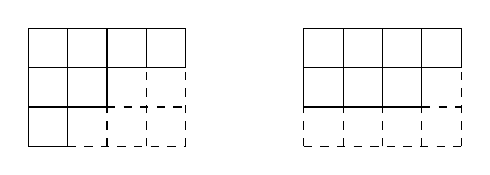
\begin{tikzpicture}[scale=0.5]
		\draw (0,3)--(4,3);
		\draw (0,2)--(4,2);
		\draw (0,1)--(2,1);
		\draw[dashed] (2,1)--(4,1);
		\draw (0,0)--(1,0);
		\draw[dashed] (1,0)--(4,0);
		\draw (0,0)--(0,3);
		\draw (1,0)--(1,3);
		\draw (2,1)--(2,3);
		\draw[dashed] (2,0)--(2,1);
		\draw (3,2)--(3,3);
		\draw[dashed] (3,0)--(3,2);
		\draw (4,2)--(4,3);
		\draw[dashed] (4,0)--(4,2);
		\draw (7,3)--(11,3);
		\draw (7,2)--(11,2);
		\draw (7,1)--(10,1);
		\draw[dashed] (10,1)--(11,1);
		\draw[dashed] (7,0)--(11,0);
		\draw[dashed] (7,0)--(7,1);
		\draw (7,1)--(7,3);
		\draw[dashed] (8,0)--(8,1);
		\draw (8,1)--(8,3);
		\draw[dashed] (9,0)--(9,1);
		\draw (9,1)--(9,3);
		\draw[dashed] (10,0)--(10,1);
		\draw (10,1)--(10,3);
		\draw[dashed] (11,0)--(11,2);
		\draw (11,2)--(11,3);
		\end{tikzpicture} \]
The continuous and broken lines show the complementary diagrams.
} This is a simple consequence of the fact that the addition of two angular momenta can give zero only if they have the same absolute magnitude.

To conclude this section, let us return to the fact already mentioned in the footnote at the end of \S\ref{The variational principle} that, for a system of several identical particles, we cannot assert that the wave function of the stationary state of lowest energy is without nodes. We can now amplify this statement and elucidate its origin.

The wave function (that is, the coordinate function), if it has no nodes, must certainly be symmetrical with respect to all the particles; for, if it were antisymmetrical with respect to the interchange of any pair of particles $ 1, 2 $, it would vanish for $ \bm{r}_1 = \bm{r}_2 $. If, however, the system consists of three or more electrons, no completely symmetrical coordinate wave function is possible (the Young diagram of the coordinate function cannot have rows with more than two cells). Thus, although the solution of Schr\"odinger’s equation which corresponds to the lowest eigenvalue is without nodes (by the theorem of the variational calculus), this solution may be physically inadmissible; the smallest eigenvalue of Schr\"odinger’s equation will not then correspond to the normal state of the system, and the wave function of this state will in general have nodes. For particles with a half-integral spin $ s $, this situation occurs in systems with more than $ 2s + 1 $ particles. For systems of bosons, a completely symmetrical coordinate wave function is always possible.





{\small
	
\textbf{PROBLEMS}


\textbf{1.}Determine the number of energy levels with different values of the total spin $ S $, for a system of $ N $ particles with spin $ 1/2 $.





SOLUTION. A given value of the projection of the total spin of the system, $ M_S = \sum \sigma $, can be obtained in
\[ f(M_S)=\frac{N!}{\left(\frac{N}{2}+M_S \right)!\left(\frac{N}{2}-M_S \right)!} \]
ways, with $ N/2 + M_S $ particles taken to have $ \sigma=1/2 $ and the remainder $ \sigma = -1/2 $. To each energy level with a given $ S $, there correspond $ 2S+1 $ states with $ M_S = S, S-1, \dots, -S $. Hence it is easy to see that the number of different energy levels with a given value of $ S $ is
\[ n(S)=f(S)-f(S+1)=\frac{N!(2S+1)}{\left(\frac{N}{2}+S+1 \right)!\left(\frac{N}{2}-S \right)!} .\]
The total number of different energy levels is
\[ n=\sum_S n(S)=f(0)=\frac{N!}{\left( \frac{N}{2}!\right)^2} \]
for even $ N $, and
\[ n=f\left(\frac{1}{2}\right)=\frac{N!}{\left(\frac{N+1}{2} \right)!\left(\frac{N-1}{2} \right)!} \]
for odd $ N $.





\textbf{2.} Find the values of the total spin $ S $ that occur for various types of symmetry of the spin functions of a system of two, three or four particles with spin $ 1 $.





SOLUTION. For two particles, the correspondence is established by the fact that the factor by which the spin function is multiplied when the particles are interchanged must be $ (-1)^{2s-S} $ (see the end of \S\ref{Exchange interaction}). For particles with spin $ s = 1 $ this gives
\begin{equation}\label{63-2-1}
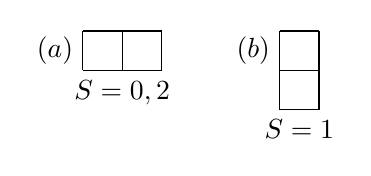
\begin{tikzpicture}[baseline,scale=0.5]
\draw (0,0)--(2,0);
\draw (0,1)--(2,1);
\draw (5,-1)--(6,-1);
\draw (5,0)--(6,0);
\draw (5,1)--(6,1);
\draw (0,0)--(0,1);
\draw (1,0)--(1,1);
\draw (2,0)--(2,1);
\draw (5,-1)--(5,1);
\draw (6,-1)--(6,1);
\node[below] at (1,0) {$ S=0,2 $};
\node[below] at (5.5,-1) {$ S=1 $};
\node[left] at (0,0.5) {$ (a) $};
\node[left] at (5,0.5) {$ (b) $}; 
\end{tikzpicture}\tag{1}
\end{equation}



The Young diagrams for a system of three particles are obtained by adding to the diagrams \eqref{63-2-1} one cell in every possible way. The result may be written as the symbolic equations
\[ 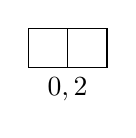
\begin{tikzpicture}[baseline,scale=0.5]
\draw (0,0)--(2,0);
\draw (0,1)--(2,1);
\draw (0,0)--(0,1);
\draw (1,0)--(1,1);
\draw (2,0)--(2,1);
\node[below] at (1,0) {$ 0,2 $};
\end{tikzpicture}\quad\times\quad\begin{tikzpicture}[baseline,scale=0.5]
\draw (0,0)--(1,0);
\draw (0,0)--(0,1);
\draw (1,0)--(1,1);
\draw (0,1)--(1,1);
\node[below] at (0.5,0) {$ 1 $};
\end{tikzpicture}\quad=\quad\underbrace{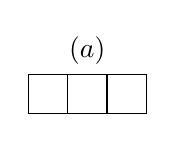
\begin{tikzpicture}[baseline,scale=0.5]
	\draw (0,0)--(3,0);
	\draw (0,0)--(0,1);
	\draw (1,0)--(1,1);
	\draw (2,0)--(2,1);
	\draw (3,0)--(3,1);
	\draw (0,1)--(3,1);
	\node[above] at (1.5,1) {$ (a) $};
	\end{tikzpicture}\quad+\quad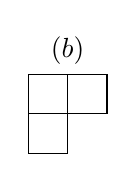
\begin{tikzpicture}[baseline,scale=0.5]
	\draw (0,0)--(2,0);
	\draw (0,-1)--(0,1);
	\draw (1,-1)--(1,1);
	\draw (2,0)--(2,1);
	\draw (0,1)--(2,1);
	\draw (2,0)--(2,1);
	\draw (0,-1)--(1,-1);
	\node[above] at (1,1) {$ (b) $};
	\end{tikzpicture}}_{1,1,2,3} \]
\[ 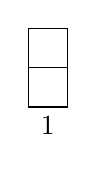
\begin{tikzpicture}[baseline,scale=0.5]
\draw (0,-1)--(0,1);
\draw (1,-1)--(1,1);
\draw (0,1)--(1,1);
\draw (0,0)--(1,0);
\draw (0,-1)--(1,-1);
\node[below] at (0.5,-1) {$ 1 $};
\end{tikzpicture}\quad\times\quad\begin{tikzpicture}[baseline,scale=0.5]
\draw (0,0)--(0,1);
\draw (1,0)--(1,1);
\draw (0,1)--(1,1);
\draw (0,0)--(1,0);
\node[below] at (0.5,-1) {$ 1 $};
\end{tikzpicture}\quad=\quad\underbrace{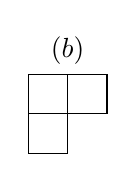
\begin{tikzpicture}[baseline,scale=0.5]
	\draw (0,-1)--(0,1);
	\draw (1,-1)--(1,1);
	\draw (2,0)--(2,1);
	\draw (0,-1)--(1,-1);
	\draw (0,0)--(2,0);
	\draw (0,1)--(2,1);
	\node[above] at (1,1) {$ (b) $};
	\end{tikzpicture}\quad+\quad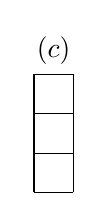
\begin{tikzpicture}[baseline,scale=0.5]
	\draw (0,-2)--(0,1);
	\draw (1,-2)--(1,1);
	\draw (0,1)--(1,1);
	\draw (0,0)--(1,0);
	\draw (0,-1)--(1,-1);
	\draw (0,-2)--(1,-2);
	\node[above] at (0.5,1) {$ (c) $};
	\end{tikzpicture}}_{0,1,2}
 \]
The values of $ S $ are shown beneath each diagram, and the values of the total spin of the system of three particles (the diagrams on the right) are found from the spins of the two-particle and one-particle systems (the diagrams on the left) by the rule of addition of angular momenta.\footnote{The repetition of $ 1 $ beneath the right-hand diagrams occurs because this value of the angular momentum comes firstly from adding the angular momenta $ 0 $ and $ 1 $, and secondly from adding $ 2 $ and $ 1 $.
} The distribution of the resulting values of $ S $ among the diagrams on the right is established by noting that diagram $ (c) $ (a column of three cells) corresponds to $ S = 0 $, and $ (b) $ therefore to the remaining values $ 1 $ and $ 2 $ in the second equation, while $ (a) $ belongs to the values $ 1 $ and $ 3 $ that are left after $ (b) $ has been labelled in the first equation:
\begin{equation}\label{63-2-2}
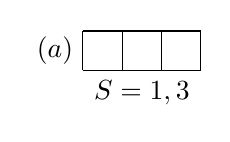
\begin{tikzpicture}[baseline,scale=0.5]
\draw (0,1)--(3,1);
\draw (0,2)--(3,2);
\draw (0,1)--(0,2);
\draw (1,1)--(1,2);
\draw (2,1)--(2,2);
\draw (3,1)--(3,2);
\node[left] at (0,1.5) {$ (a) $};
\node[below] at (1.5,1) {$ S=1,3 $};
\end{tikzpicture}\qquad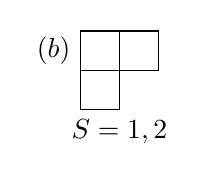
\begin{tikzpicture}[baseline,scale=0.5]
\draw (0,1)--(2,1);
\draw (0,2)--(2,2);
\draw (0,0)--(1,0);
\draw (0,0)--(0,2);
\draw (1,0)--(1,2);
\draw (2,1)--(2,2);
\node[left] at (0,1.5) {$ (b) $};
\node[below] at (1,0) {$ S=1,2 $};
\end{tikzpicture}\qquad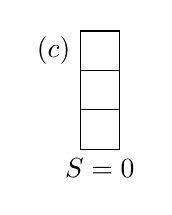
\begin{tikzpicture}[baseline,scale=0.5]
\draw (0,-1)--(0,2);
\draw (1,-1)--(1,2);
\draw (0,-1)--(1,-1);
\draw (0,0)--(1,0);
\draw (0,1)--(1,1);
\draw (0,2)--(1,2);
\node[left] at (0,1.5) {$ (c) $};
\node[below] at (0.5,-1) {$ S=0 $};
\end{tikzpicture}\tag{2}
\end{equation}
The Young diagrams for a system of four particles are obtained by adding one cell to the diagrams \eqref{63-2-2}, with the condition that no column should contain more than three cells:
\begin{equation*}
\begin{split}
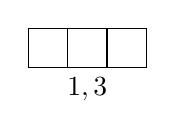
\begin{tikzpicture}[baseline,scale=0.5]
\draw (0,0)--(3,0);
\draw (0,1)--(3,1);
\draw (0,0)--(0,1);
\draw (1,0)--(1,1);
\draw (2,0)--(2,1);
\draw (3,0)--(3,1);
\node[below] at (1.5,0) {$ 1,3 $};
\end{tikzpicture}\quad\times\quad\begin{tikzpicture}[baseline,scale=0.5]
\draw (0,0)--(0,1);
\draw (0,1)--(1,1);
\draw (1,0)--(1,1);
\draw (0,0)--(1,0);
\node[below] at (0.5,0) {$ 1 $};
\end{tikzpicture}\quad&=\quad\underbrace{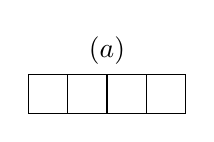
\begin{tikzpicture}[baseline,scale=0.5]
	\draw (0,0)--(4,0);
	\draw (0,1)--(4,1);
	\draw (0,0)--(0,1);
	\draw (1,0)--(1,1);
	\draw (2,0)--(2,1);
	\draw (3,0)--(3,1);
	\draw (4,0)--(4,1);
	\node[above] at (2,1) {$ (a) $};
	\end{tikzpicture}\quad+\quad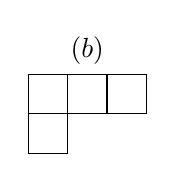
\begin{tikzpicture}[baseline,scale=0.5]
	\draw (0,0)--(3,0);
	\draw (0,1)--(3,1);
	\draw (0,-1)--(1,-1);
	\draw (0,-1)--(0,1);
	\draw (1,-1)--(1,1);
	\draw (2,0)--(2,1);
	\draw (3,0)--(3,1);
	\node[above] at (1.5,1) {$ (b) $};
	\end{tikzpicture}}_{0,1,2,2,3,4}\\
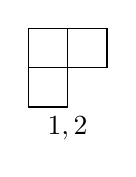
\begin{tikzpicture}[baseline,scale=0.5]
\draw (0,0)--(2,0);
\draw (0,1)--(2,1);
\draw (0,-1)--(1,-1);
\draw (0,-1)--(0,1);
\draw (1,-1)--(1,1);
\draw (2,0)--(2,1);
\node[below] at (1,-1) {$ 1,2 $}; 
\end{tikzpicture}\quad\times\quad\begin{tikzpicture}[baseline,scale=0.5]
\draw (0,0)--(1,0);
\draw (1,0)--(1,1);
\draw (0,1)--(1,1);
\draw (0,0)--(0,1);
\node[below] at (0.5,-1) {$ 1 $};
\end{tikzpicture}\quad&=\quad\underbrace{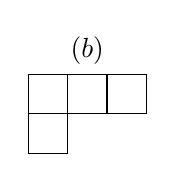
\begin{tikzpicture}[baseline,scale=0.5]
	\draw (0,0)--(3,0);
	\draw (0,1)--(3,1);
	\draw (0,-1)--(1,-1);
	\draw (0,-1)--(0,1);
	\draw (1,-1)--(1,1);
	\draw (2,0)--(2,1);
	\draw (3,0)--(3,1);
	\node[above] at (1.5,1) {$ (b) $};
	\end{tikzpicture}\quad+\quad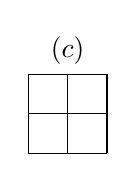
\begin{tikzpicture}[baseline,scale=0.5]
	\draw (0,0)--(2,0);
	\draw (0,1)--(2,1);
	\draw (0,-1)--(2,-1);
	\draw (0,-1)--(0,1);
	\draw (1,-1)--(1,1);
	\draw (2,-1)--(2,1);
	\node[above] at (1,1) {$ (c) $};
	\end{tikzpicture}\quad+\quad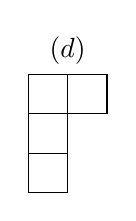
\begin{tikzpicture}[baseline,scale=0.5]
	\draw (0,0)--(2,0);
	\draw (0,1)--(2,1);
	\draw (0,-1)--(1,-1);
	\draw (0,-2)--(1,-2);
	\draw (0,-2)--(0,1);
	\draw (1,-2)--(1,1);
	\draw (2,0)--(2,1);
	\node[above] at (1,1) {$ (d) $};
	\end{tikzpicture}}_{0,1,1,2,2,3}\\
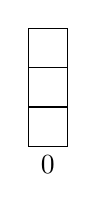
\begin{tikzpicture}[baseline,scale=0.5]
\draw (0,-2)--(0,1);
\draw (1,-2)--(1,1);
\draw (0,-2)--(1,-2);
\draw (0,-1)--(1,-1);
\draw (0,0)--(1,0);
\draw (0,1)--(1,1);
\node[below] at (0.5,-2) {$ 0 $};
\end{tikzpicture}\quad\times\quad\begin{tikzpicture}[baseline,scale=0.5]
\draw (0,0)--(1,0);
\draw (0,0)--(0,1);
\draw (1,0)--(1,1);
\draw (0,1)--(1,1);
\node[below] at (0.5,0) {$ 1 $};
\end{tikzpicture}\quad&=\quad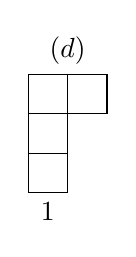
\begin{tikzpicture}[baseline,scale=0.5]
\draw (0,1)--(2,1);
\draw (0,0)--(2,0);
\draw (0,-1)--(1,-1);
\draw (0,-2)--(1,-2);
\draw (0,-2)--(0,1);
\draw (1,-2)--(1,1);
\draw (2,0)--(2,1);
\node[above] at (1,1) {$ (d) $};
\node[below] at (0.5,-2) {$ 1 $};
\end{tikzpicture}
\end{split}
\end{equation*}
Diagram $ (c) $ can be added to $ (a) $ in $ (1) $ to form a rectangle with three-cell columns, and therefore corresponds to the same values $ S = 0, 2 $. The values of $ S $ for diagram $ (b) $ are found from the remainder of the second equation, and then those for $ (a) $ from the remainder of the first equation:
\[ 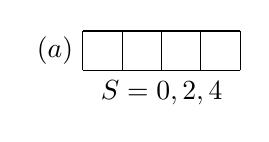
\begin{tikzpicture}[baseline,scale=0.5]
\draw (0,0)--(4,0);
\draw (0,1)--(4,1);
\draw (0,0)--(0,1);
\draw (1,0)--(1,1);
\draw (2,0)--(2,1);
\draw (3,0)--(3,1);
\draw (4,0)--(4,1);
\node[left] at (0,0.5) {$ (a) $};
\node[below] at (2,0) {$ S=0,2,4 $};
\end{tikzpicture}\qquad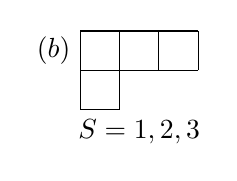
\begin{tikzpicture}[baseline,scale=0.5]
\draw (0,0)--(3,0);
\draw (0,1)--(3,1);
\draw (0,-1)--(1,-1);
\draw (0,-1)--(0,1);
\draw (1,-1)--(1,1);
\draw (2,0)--(2,1);
\draw (3,0)--(3,1);
\node[left] at (0,0.5) {$ (b) $};
\node[below] at (1.5,-1) {$ S=1,2,3 $};
\end{tikzpicture}\qquad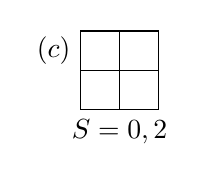
\begin{tikzpicture}[baseline,scale=0.5]
\node[left] at (0,0.5) {$ (c) $};
\draw (0,1)--(2,1);
\draw (0,0)--(2,0);
\draw (0,-1)--(2,-1);
\draw (0,-1)--(0,1);
\draw (1,-1)--(1,1);
\draw (2,-1)--(2,1);
\node[below] at (1,-1) {$ S=0,2 $};
\end{tikzpicture}\qquad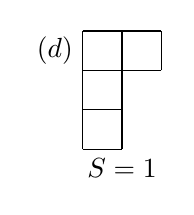
\begin{tikzpicture}[baseline,scale=0.5]
\draw (0,0)--(2,0);
\draw (0,1)--(2,1);
\draw (0,-1)--(1,-1);
\draw (0,-2)--(1,-2);
\draw (0,-2)--(0,1);
\draw (1,-2)--(1,1);
\draw (2,0)--(2,1);
\node[left] at (0,0.5) {$ (d) $};
\node[below] at (1,-2) {$ S=1 $};
\end{tikzpicture} \]
}
\section{Second quantization. The case of Bose statistics}\label{Second quantization. The case of Bose statistics}
In the theory of systems consisting of a large number of identical particles, there is a widely used method of considering the problem, known as \textit{second quantization}. This method is especially necessary in relativistic theory, where we have to deal with systems in which the number of particles is itself variable.\footnote{The method of second quantization was developed by P. A. M. Dirac (1927) for photons in radiation theory, and later extended to fermions by E. Wigner and P. Jordan (1928).
}

Let $ \psi_1(\xi), \psi_2(\xi), \dots $ be some complete set of orthogonal and normalized wave functions of stationary states of a single particle.\footnote{As in \S\ref{The principle of indistinguishability of similar particles}, $\xi$ denotes the set of the coordinates and the spin projection $\sigma$ of the particle, and integration with respect to $\xi$ is taken to mean integration over the coordinates and summation over $\sigma$.
} These may be states of a particle in some arbitrarily chosen external field, but are usually taken to be simply plane waves, i.e. the wave functions of a free-particle having definite values of the momentum (and spin projection). In order to make the spectrum of states discrete, we shall consider the motion of particles in a large but finite region, for which the eigenvalues of the momentum components form a discrete series, the intervals between adjacent values being inversely proportional to the linear dimensions of the region and tending to zero as these increase.

In a system of free particles, the particle momenta are separately conserved. The occupation numbers of the states are therefore also conserved, i.e. the numbers $ N_1, N_2, \dots $ which show how many particles are in each of the states $ \psi_1, \psi_2, \dots $. In a system of interacting particles, the momentum of each particle is not conserved, and so the occupation numbers are not conserved. For such a system we can consider only the probability distribution of the various values of the occupation numbers. Let us seek to construct a mathematical formalism in which the occupation numbers (and not the coordinates and spin projections of the particles) play the part of independent variables.

In this formalism, it is convenient to use the Dirac notation (see the end of \S\ref{Matrices}), taking $ N_1, N_2, \dots $ as quantum numbers defining the state. The states corresponding to the wave functions \eqref{61.3} and \eqref{61.5} will be denoted by $ \left|N_1, N_2, \dots\> $. The coordinate and spin variables of the particles are not shown explicitly.

In accordance with this choice of the independent variables, the operators of the various physical quantities (including the Hamiltonian of the system) must be formulated in terms of their action on functions of the occupation numbers. Such a formulation can be obtained on the basis of the usual matrix representation of operators. The operator matrix elements must be considered in relation to the wave functions of the stationary states of a system of non-interacting particles. Since these states can be described by specifying definite values of the occupation numbers, this will also show the nature of the action of the operators on these variables.

Let us first consider systems of particles obeying Bose statistics. Let $ \hat{f}_a^{(1)} $ be the operator of some quantity pertaining to the $ a $th particle, i.e. acting only on functions of the variables $\xi_a$. We introduce the operator
\begin{equation}\label{64.1}
\hat{F}^{(1)}=\sum_a\hat{f}_a^{(1)}
\end{equation}
which is symmetrical with respect to all the particles (the summation being over all particles), and determine its matrix elements with respect to the wave functions \eqref{61.3}. First of all, it is easy to see that the matrix elements will be different from zero only for transitions which leave the numbers $ N_1, N_2, \dots $ unchanged (diagonal elements) and for transitions where one of these numbers is increased, and another decreased, by unity. For, since each of the operators $ \hat{f}_a^{(1)} $ acts only on one function in the product $ \psi_{p_1}(\xi_1)\psi_{p_2}(\xi_2)\dots \psi_{p_N}(\xi_N) $, its matrix elements can be different from zero only for transitions whereby the state of a single particle is changed; this, however, means that the number of particles in one state is diminished by unity, while the number in another state is correspondingly increased. The calculation of these matrix elements is in principle very simple; it is easier to do it oneself than to follow an account of it. Hence we shall give only the result of this calculation. The non-diagonal elements are
\begin{equation}\label{64.2}
\< N_i,N_k-1|F^{(1)}|N_i-1,N_k\>=f_{ik}^{(1)}\sqrt{N_iN_k}.
\end{equation}
We shall indicate only those suffixes with respect to which the matrix element is non-diagonal, omitting the remainder for brevity. Here $ f_{ik}^{(1)} $ is the matrix element
\begin{equation}\label{64.3}
f_{ik}^{(1)}=\int\psi_i^*(\xi)\hat{f}^{(1)}\psi_k(\xi)\d\xi;
\end{equation}
since the operators $ f_a^{(1)} $ differ only in the naming of the variables on which they act, the integrals \eqref{64.3} are independent of a, which is therefore omitted. The diagonal matrix elements of $ F^{(1)} $ are the mean values of the quantity $ F^{(1)} $ in the states $ \Psi_{N_1N_2\dots} $. Calculation gives
\begin{equation}\label{64.4}
\bar{F^{(1)}}=\sum_i f_{ii}^{(1)}N_i.
\end{equation}



We now introduce the operators $ \hat{a}_i $, which play a leading part in the method of second quantization; they act, not on functions of the coordinates, but on functions of the occupation numbers. By definition, the operator $ \hat{a}_i $ acting on the function $ \left|N1, N2, \dots\> $ decreases the value of the variable $ N_i $ by unity, and at the same time it multiplies the function by $\sqrt{N_i}$:\footnote{Here we use the notation $ \hat{a}\left|m\> $ with the natural sense of the result of the operator $\hat{a}$ acting on the state wave function $ \left|m\>. $
}
\begin{equation}\label{64.5}
\hat{a}_i\left|N_1,N_2,\dots,N_i,\dots\>=\sqrt{N_i}\left|N_1,N_2,\dots,N_i-1,\dots\>.
\end{equation}
We can say that the operator $\hat{a}_i$ diminishes by one the number of particles in the $ i $th state; it is therefore called a particle \textit{annihilation operator}. It can be represented in the form of a matrix whose only non-zero element is
\begin{equation}\label{64.6}
\< N_i-1|a_i|N_i\>=\sqrt{N_i}.
\end{equation}


The operator $ \hat{a}_i^\dagger $ which is the Hermitian conjugate of $ \hat{a}_i $ is, by definition (see \eqref{11.9}), represented by a matrix whose only non-zero element is
\begin{equation}\label{64.7}
\<N_i\right|a_i^\dagger\left|N_i-1\>=\<N_i-1|a_i|N_i\>^*=\sqrt{N_i}
\end{equation}
This means that, when acting on the function $ \Phi(N_1, N_2, \dots) $. it increases the number $ N_i $ by unity:
\begin{equation}\label{64.8}
\hat{a}_i^\dagger\left|N_1,N_2,\dots,N_i,\dots\>=\sqrt{N_i+1}\left|N_1,N_2,\dots,N_i+1,\dots\>.
\end{equation}
In other words, the operator $\hat{a}_i^\dagger$ increases by one the number of particles in the $ i $th state, and is therefore called a particle \textit{creation operator}.

The product of the operators $ \hat{a}_i^\dagger\hat{a}_i $, acting on the wave function, must multiply it by a constant simply, leaving unchanged all the variables $ N_1, N_2, \dots $: the operator $\hat{a}_i$ diminishes $ N_i $ by unity, and $\hat{a}_i^\dagger$ then restores it to its original value. Direct multiplication of the matrices \eqref{64.6} and \eqref{64.7} shows that $ \hat{a}_i^\dagger\hat{a}_i $ is represented, as we should expect, by a diagonal matrix whose diagonal elements are $ N_i $. We can write
\begin{equation}\label{64.9}
 \hat{a}_i^\dagger\hat{a}_i =N_i.
\end{equation}
Similarly, we find that
\begin{equation}\label{64.10}
\hat{a}_i\hat{a}_i^\dagger=N_i+1.
\end{equation}



The difference of these equations gives the commutation rule for the operators $\hat{a}_i$ and $ \hat{a}_i^\dagger $:
\begin{equation}\label{64.11}
\hat{a}_i\hat{a}_i^\dagger-\hat{a}_i^\dagger\hat{a}_i=1.
\end{equation}
The operators with $ i $ and $ k $ different act on different variables ($ N_i $ and $ N_k $), and commute:
\begin{equation}\label{64.12}
\hat{a}_i\hat{a}_k-\hat{a}_k\hat{a}_i=0,\quad\hat{a}_i\hat{a}_k^\dagger-\hat{a}_k^\dagger\hat{a}_i=0,\quad i\ne k.
\end{equation}



From the above properties of the operators $ \hat{a}_i, \hat{a}_i^\dagger $ it is easy to see that the operator
\begin{equation}\label{64.13}
\hat{F}^{(1)}=\sum_{i,k}=f_{ik}^{(1)}\hat{a}_i^\dagger\hat{a}_k
\end{equation}
is the same as the operator \eqref{64.1}. For all the matrix elements calculated from \eqref{64.6}, \eqref{64.7} are the same as the elements \eqref{64.2}, \eqref{64.4}. This is a very important result. In formula \eqref{64.13}, the quantities $ f^{(1)}_{ik} $ are simply numbers. Thus we have been able to express an ordinary operator, acting on functions of the coordinates, in the form of an operator acting on functions of new variables, the occupation numbers $ N_i $.

The result which we have obtained is easily generalized to operators of other forms. Let
\begin{equation}\label{64.14}
\hat{F}^{(2)}=\sum_{a>b}\hat{f}_{ab}^{(2)},
\end{equation}
where $ \hat{f}_{ab}^{(2)} $ is the operator of a physical quantity pertaining to two particles at once, and hence acts on functions of $\xi_a$ and $\xi_b$. Similar calculations show that this operator can be expressed in terms of the operators $ \hat{a}_i, \hat{a}_i^\dagger $ by
\begin{equation}\label{64.15}
\hat{F}^{(2)}=\frac{1}{2}\sum_{i,k,l,m}\< ik|f^{(2)}|lm\>\hat{a}_i^\dagger\hat{a}_k^\dagger\hat{a}_m\hat{a}_l,
\end{equation}
where
\[ \< ik|f^{(2)}|lm\>=\iint\psi_i^*(\xi_1)\psi_k^*(\xi_2)\hat{f}^{(2)}\psi_l(\xi_1)\psi_m(\xi_2)\d\xi_1\d\xi_2. \]
The generalization of these formulae to operators of any other form symmetrical with respect to all the particles (of the form $ \hat{F}^{(3)} = \sum\hat{f}^{(3)}_{abc} $, etc.) is obvious.

These formulae can be used to express, in terms of the operators $\hat{a}_i$ and $\hat{a}_i^\dagger$, the Hamiltonian of the physical system of $ N $ identical interacting particles that is being considered. The Hamiltonian of such a system is, of course, symmetrical with respect to all the particles. In the non-relativistic approximation,\footnote{n the absence of a magnetic field.} it is independent of the spins of the particles, and can be represented in a general form as follows:
\begin{equation}\label{64.16}
\hat{H}=\sum_a\hat{H}_a^{(1)}+\sum_{a>b}U^{(2)}(\bm{r}_a,\bm{r}_b)+\sum_{a>b>c}U^{(3)}(\bm{r}_a,\bm{r}_b,\bm{r}_c)+\dots
\end{equation}
Here $ \hat{H}^{(1)}_a $ is the part of the Hamiltonian which depends on the coordinates of the $ a $th particle only:
\begin{equation}\label{64.17}
\hat{H}_a^{(1)}=-\frac{\h^2}{2m}\Delta_a+U^{(1)}(\bm{r}_a).
\end{equation}
where $ U^{(1)}(\bm{r}_a) $ is the potential energy of a single particle in the external field. The remaining terms in \eqref{64.16} correspond to the mutual interaction energy of the particles; the terms depending on the coordinates of two, three, etc. particles have been separated.

This representation of the Hamiltonian enables us to apply formulae \eqref{64.13}, \eqref{64.15} and their analogues directly. Thus
\begin{equation}\label{64.18}
\hat{H}=\sum_{i,k}H_{ik}^{(1)}\hat{a}_i^\dagger\hat{a}_k+\frac{1}{2}\sum_{i,k,l,m}\< ik|U^{(2)}|lm\>\hat{a}_i^\dagger\hat{a}_k^\dagger\hat{a}_m\hat{a}_l\dots
\end{equation}
This gives the required expression for the Hamiltonian in the form of an operator acting on functions of the occupation numbers.

For a system of non-interacting particles, only the first term in the expression \eqref{64.18} remains:
\begin{equation}\label{64.19}
\hat{H}=\sum_{i,k}H_{ik}^{(1)}\hat{a}_i^\dagger\hat{a}_k.
\end{equation}
If the functions $\psi_i$ are taken to be the eigenfunctions of the Hamiltonian $ \hat{H}^{(1)} $ of an individual particle, the matrix $ \hat{H}^{(1)}_{ik} $ is diagonal, and its diagonal elements are the eigenvalues $ \epsilon_i $ of the energy of the particle. Thus,
\[ \hat{H}=\sum_i\epsilon_i\hat{a}_i^\dagger\hat{a}_i; \]
replacing the operator $ \hat{a}_i^\dagger\hat{a}_i $ by its eigenvalues \eqref{64.9}, we have for the energy levels of the system the expression
\[ E=\sum_i\epsilon_i N_i \]
a trivial result which could have been foreseen.

The formalism which we have developed can be put in a more compact form by introducing the $\psi$-\textit{operators}\footnote{Note the analogy between \eqref{64.20} and the expansion
\[ \psi=\sum a_i\psi_i \]	
of any wave function in terms of a complete set of functions. Here it is “re-quantized”, and this is the reason for the term \textit{second quantization method}.}
\begin{equation}\label{64.20}
\hat{\psi}(\xi)=\sum_i\psi_i(\xi)\hat{a}_i\quad\hat{\psi}^\dagger(\xi)=\sum_i\psi^*(\xi)\hat{a}_i^\dagger,
\end{equation}
where the variables $\xi$ are regarded as parameters. By what has been said above concerning the operators $ \hat{a}_i, \hat{a}_i^\dagger $, it is clear that the operator $\hat{\psi}$ decreases the total number of particles in the system by one, while $\hat{\psi}^\dagger$ increases it by one.

It is easy to see that the operator $ \hat{\psi}^\dagger(\xi_0) $ creates a particle at the point $\xi_0$. For the result of the action of the operator $\hat{a}_i^\dagger$ is to create a particle in a state with wave function $\psi_i(\xi)$. Hence it follows that the result of the action of the operator $ \hat{\psi}^\dagger(\xi_0) $ is to create a particle in a state with wave function \[ \sum_i\psi_i^*(\xi)\psi_i(\xi_0)=\delta(\xi-\xi_0) , \] 
which corresponds to a particle with definite values of the coordinates (and spin). Here we have used formula \eqref{5.12}.\footnote{$ \delta(\xi-\xi_0) $ conventionally denotes the product
\[ \delta(x-x_0)\delta(y-y_0)\delta(z-z_0)\delta_{\sigma\sigma_0}. \]}

The commutation rules for the $\psi$ operators are obtained at once from those for the operators $ \hat{a}_i, \hat{a}_i^\dagger $:
\begin{equation}\label{64.21}
\hat{\psi}(\xi)\hat{\psi}(\xi')-\hat{\psi}(\xi')\hat{\psi}(\xi)=0,
\end{equation}
\begin{equation}\label{64.22}
\hat{\psi}(\xi)\hat{\psi}^\dagger(\xi')-\hat{\psi}^\dagger(\xi')\hat{\psi}(\xi)=\sum_i\psi_i(\xi)\psi_i^*(\xi')=\delta(\xi-\xi').
\end{equation}




The second-quantized operator $ \hat{F}^{(1)} $ can be written by means of the $\psi$ operators in the form
\begin{equation}\label{64.23}
\hat{F}^{(1)}=\int\hat{\psi}^\dagger(\xi)\hat{f}^{(1)}\hat{\psi}(\xi)\d\xi
\end{equation}
where it is understood that the operator $ \hat{f}^{(1)} $ acts on functions of the parameters $\xi$ in $\hat{\psi}(\xi)$. For, substituting $\hat{\psi}$ and $\hat{\psi}^\dagger$ in the form \eqref{64.20} and using the definition \eqref{64.3}, we return to \eqref{64.13}. Similarly, \eqref{64.15} becomes
\begin{equation}\label{64.24}
\hat{F}^{(2)}=\frac{1}{2}\iint\hat{\psi}^\dagger(\xi)\hat{\psi}^\dagger(\xi')\hat{f}^{(2)}\hat{\psi}(\xi')\hat{\psi}(\xi)\d\xi\d\xi'.
\end{equation}



In particular, the Hamiltonian of the system, expressed in terms of the $\psi$ operators, is
\begin{multline}\label{64.25}
\hat{H}=\int\left\{-\frac{\h^2}{2m}\hat{\psi}^\dagger(\xi)\Delta\hat{\psi}(\xi)+\hat{\psi}^\dagger(\xi)U^{(1)}(\xi)\hat{\psi}(\xi) \right\}\d\xi+\\
+\frac{1}{2}\iint\hat{\psi}^\dagger(\xi)\hat{\psi}^\dagger(\xi')U^{(2)}(\xi,\xi')\hat{\psi}(\xi')\hat{\psi}(\xi)\d\xi\d\xi'+\dots
\end{multline}



The operator $ \hat{\psi}^\dagger(\xi)\hat{\psi}(\xi) $, constructed from the $\psi$ operators by analogy with the product $ \psi^*\psi $ which determines the probability density for a particle in a state with wave function $\psi$, is called the \textit{particle density operator}. The integral
\begin{equation}\label{64.26}
\hat{N}=\int\hat{\psi}^\dagger\hat{\psi}\d\xi
\end{equation}
represents in the second-quantization formalism the operator of the total number of particles in the system. For, substituting the $\psi$ operators in the form \eqref{64.20} and using the normalization and the orthogonality of the wave functions, we have
\[ \hat{N}=\sum\hat{a}_i^\dagger\hat{a}_i. \]
Each term in this sum is the operator of the number of particles in the ith state; according to \eqref{64.9}, its eigenvalues are equal to the occupation numbers $ N_i $, and the sum of all these numbers is the total number of particles in the system.\footnote{For systems containing a specified number of particles these statements are trivial, as are the properties of the Hamiltonian \eqref{64.19} of a system of free particles. Their generalization in the relativistic theory, however, yields new results that are by no means trivial (cf. RQT, \S11)
}

Lastly, if the system consists of bosons of various kinds, operators $\hat{a}$ and $\hat{a}^\dagger$ for each kind of particle must be defined in the second quantization method. It is evident that operators pertaining to particles of different kinds commute.
\section{Second quantization. The case of Fermi statistics}\label{Second quantization. The case of Fermi statistics}
The basic theory of the method of second quantization remains wholly unchanged for systems of identical fermions, but the actual formulae for the matrix elements of quantities and for the operators $ \hat{a}_i $ are naturally different.

The wave function $ \psi_{N_1N_2\dots} $ now has the form \eqref{61.5}. Because of the antisymmetry of this function, the question of its sign arises first of all. This question did not arise in the case of Bose statistics, since, because of the symmetry of the wave function, its sign, once chosen, was preserved under all permutations of the particles. In order to make definite the sign of the function \eqref{61.5}, we shall agree to choose it as follows. We number successively, once and for all, all the states $\psi_i$. We then complete the rows of the determinant \eqref{61.5} so that always
\begin{equation}\label{65.1}
p_1<p_2<p_3<\dots<p_N,
\end{equation}
whilst in the successive columns we have functions of the different variables in the order $ \xi_1,\xi_2,\dots,\xi_N $. No two of the numbers $ p_1, p_2, \dots $ can be equal, since otherwise the determinant would vanish. In other words, the occupation numbers $ N_i $ can take only the values $ 0 $ and $ 1 $.

Let us again consider an operator of the form \eqref{64.1}, $ \hat{F}^{(1)}=\sum\hat{f}_a^{(1)} $. As in \S\ref{Second quantization. The case of Bose statistics}, its matrix elements will be non-zero only for transitions where all the occupation numbers remain unchanged and for those where one occupation number $ (N_i) $ is diminished by unity (becoming zero instead of one) and another $ (N_k) $ is increased by unity (becoming one instead of zero). We easily find that, for $ i < k $,
\begin{equation}\label{65.2}
\<1_i,0_k|F^{(1)}|0_i,1_k\>=f_{ik}^{(1)}(-1)^{\sum(i+1,k-1)}.
\end{equation}
where by $ 0_i, 1_i $ we signify $ N_i = 0 $, $ N_i = 1 $ and the symbol $ \sum(k,l) $ denotes the sum of the occupation numbers of all states from the $ k $th to the $ l $th:\footnote{For $ i > k $ the exponent in \eqref{65.2} becomes $ \sum(k+1,i-1) $. The sum must be taken as zero when $ i = k\pm1 $.}
\[ \sum(k,l)=\sum_{n=k}^l N_n. \]
For the diagonal elements we obtain our previous formula \eqref{64.4}:
\begin{equation}\label{65.3}
\bar{F^{(1)}}=\sum_i f_{ii}^{(1)}N_i
\end{equation}



In order to represent the operator $ \hat{F}^{(1)} $ in the form \eqref{64.13}, the operators $\hat{a}_i$ must be defined as matrices whose elements are
\begin{equation}\label{65.4}
\<0_i|a_i|1_i\>=\<1_i\right|a_i^\dagger\left|0_i\>=(-1)^{\sum(1,i-1)}.
\end{equation}
On multiplying these matrices, we find, for $ k > i $,
\begin{multline*}
\<1_i,0_k\right|a_i^\dagger a_k\left|0_i,1_k\>=\<1_i,0_k\right|a_i^\dagger\left|0_i,0_k\>\<0_i,0_k|a_k|0_i,1_k\>=\\
=(-1)^{\sum(1,i-1)}(-1)^{\sum(1,i-1)+\sum(i+1,k-1)}
\end{multline*}
or
\begin{equation}\label{65.5}
\<1_i,0_k\right|a_i^\dagger a_k\left|0_i,1_k\>=(-1)^{\sum(i+1,k-1)}.
\end{equation}
If $ i = k $, the matrix of $ \hat{a}_i^\dagger\hat{a}_i $ is diagonal, and its elements are unity for $ N_i = 1 $, and zero for $ N_i = 0 $; this can be written
\begin{equation}\label{65.6}
\hat{a}_i^\dagger\hat{a}_i=N_i.
\end{equation}
On substituting these expressions in \eqref{64.13}, we in fact obtain \eqref{65.2}, \eqref{65.3}.

Multiplying $ \hat{a}_i^\dagger, \hat{a}_k $ in the opposite order, we have
\begin{multline*}
\<1_i,0_i\right|a_k\hat{a}_i^\dagger\left|0_i,1_k\>=\<1_i,0_k|a_k|1_i,1_k\>\<1_i,1_k\right|a_i^\dagger\left|0_i,1_k\>=\\
=(-1)^{\sum(1,i-1)+\sum(i+1,k-1)+\sum(1,i-1)+1}
\end{multline*}
or
\begin{equation}\label{65.7}
\<1_i,0_k\right|a_ka_i^\dagger\left|0_i,1_k\>=-(-1)^{\sum(i+1,k-1)}.
\end{equation}
Comparing \eqref{65.7} with \eqref{65.5}, we see that these quantities have opposite signs, i.e.
\[ \hat{a}_i\hat{a}_k^\dagger+\hat{a}_k\hat{a}_i^\dagger=0,\quad i\ne k. \]



For the diagonal matrix $ \hat{a}_i\hat{a}_i^\dagger $, we find
\begin{equation}\label{65.8}
\hat{a}_i\hat{a}_i^\dagger=1-N_i
\end{equation}
Adding this to \eqref{65.6}, we obtain
\[ \hat{a}_i\hat{a}_i^\dagger+\hat{a}_i^\dagger\hat{a}_i=1.\]
Both the above equations can be written in the form
\begin{equation}\label{65.9}
\hat{a}_i\hat{a}_k^\dagger+\hat{a}_k^\dagger\hat{a}_i=\delta_{ik}.
\end{equation}
On carrying out similar calculations, we find for the products $ \hat{a}_i\hat{a}_k $ the relations
\begin{equation}\label{65.10}
\hat{a}_i\hat{a}_k+\hat{a}_k\hat{a}_i=0,
\end{equation}
and in particular $\hat{a}_i\hat{a}_i = 0 $.

Thus we see that the operators $ \hat{a}_i $ and $ \hat{a}_k $ (or $\hat{a}_k^\dagger$) for $ i\ne k $ anticommute, whereas in the case of Bose statistics they commuted with one another. This difference is perfectly natural. In the case of Bose statistics, the operators $\hat{a}_i$ and $\hat{a}_k$ were completely independent; each of the operators $\hat{a}_i$ acted only on a single variable $ N_i $, and the result of this action did not depend on the values of the other occupation numbers. In the case of Fermi statistics, however, the result of the action of the operator $\hat{a}_i$ depends not only on the number $ N_i $ itself, but also on the occupation numbers of all the preceding states, as we see from the definition \eqref{65.4}. Hence the action of the various operators $ \hat{a}_i,\hat{a}_k $ cannot be considered independent.

The properties of the operators $ \hat{a}_i,\hat{a}_i^\dagger $ having been thus defined, all the remaining formulae \eqref{64.13}--\eqref{64.18} remain valid. The formulae \eqref{64.23}--\eqref{64.25}, which express the operators of physical quantities in terms of the $\psi$-operators defined by \eqref{64.20}, also hold good. The commutation rules \eqref{64.21}, \eqref{64.22}, however, are now replaced by
\begin{equation}\label{65.11}
\hat{\psi}^\dagger(\xi')\hat{\psi}(\xi)+\hat{\psi}(\xi)\hat{\psi}^\dagger(\xi')=\delta(\xi-\xi'),
\end{equation}
\begin{equation}\label{65.12}
\hat{\psi}(\xi')\hat{\psi}(\xi)+\hat{\psi}(\xi)\hat{\psi}(\xi')=0.
\end{equation}





If the system consists of particles of different kinds, second quantization operators must be defined for each kind of particle (as already mentioned at the end of §64). Operators belonging to bosons and fermions commute; those belonging to different fermions may formally be regarded as either commutative or anticommutative within the limits of non-relativistic theory. On either assumption the results obtained by means of the second quantization method are the same.

However, with a view to later applications in the relativistic theory, which allows different particles to be transformed into one another, we should assume that the creation and annihilation operators for different fermions anticommute. This becomes evident if we regard as “different” particles two different internal states of a single complex particle.









